\documentclass[oneside,english]{scrbook}
\usepackage[T1]{fontenc}
\usepackage[latin9]{inputenc}
\setcounter{secnumdepth}{3}
\setcounter{tocdepth}{3}

\usepackage{graphicx}
\usepackage{hyperref}

\makeatletter
%%%%%%%%%%%%%%%%%%%%%%%%%%%%%% Textclass specific LaTeX commands.
\newenvironment{lyxcode}
{\par\begin{list}{}{
\setlength{\rightmargin}{\leftmargin}
\setlength{\listparindent}{0pt}% needed for AMS classes
\raggedright
\setlength{\itemsep}{0pt}
\setlength{\parsep}{0pt}
\normalfont\ttfamily}%
 \item[]}
{\end{list}}

\makeatother

\usepackage{babel}
\usepackage{listings}

\begin{document}
\title{Linux Multimedia Programming}
\author{Graphics, Audio, Video}
\date{Curator: Charles Fox}
\publishers{Licence: CC-BY-SA 3.0}
\maketitle

\chapter*{Licence}

This text uses Creative Commons licence CC-BY-SA 3.0 to ensure its continual free distribution and use of material by others. The text is made by automatically including read compilable program files, which are also CC-BY-SA 3.0 licenced and stored together with it on github. Each program lives in its own directory with its own CMake file.  It uses material from Wikipedia, www.wikipedia.org, which is released under the CC-BY-SA 3.0 licence. As a condition of CC-BY-SA, the first (title) page and this section must not be modified.  This text remixes material from many articles which can be listed by searching www.wikipedia.org for this text.  Wikipedia author names and contribution logs may be found on these articles' history pages.   The nature of computing cookbooks such as this is that short code and text quotations are often passed around between websites and documents and it is not always possible to fully trace their origins. If you are the author of such code or text and do not wish it to be used here then please let the authors know so it can be removed. 
Current authors include: Charles Fox, ADD NAMES HERE

\tableofcontents

\chapter{Introduction}

This is my first attempt at open sourcing some written notes using github and Creative Commons like what my friend Robin Lovelace does. I am collecting all my little text files and code snippits from over the years of working with Linux graphics, sound and video into one place and thought I might as well share them in case they are useful to anyone.  As I just finished writing my Springer book "Data Science for Transport" it's easy to reuse the book template, though this is just intended as a loose collection of stuff, not an actual book itself.

The idea is to select only the best of breed of everything and present them together. It's like a Linux distribution in making these selections. But it is a distribution of ideas and choices rather than of actual software. (unless we do a Docker as well).   As such, the choice of what to leave out and not cover is also important. The idea is to present a single, best, toolkit, of tools which work and which also work well with one another as in a distro.

It is not a detailed tech manual. The purpose is to present the best tools for media tasks, and to give basic but compilable hello-world examples of code to help get new project started. I use these code snippets all the time when I need to make small new projects based on libraries I might not have used for a while and need to remember how to set them up.  After that it's usually easy to consult their big docs on the net to get details for the specific things I need to do.

Maybe one day this might get big enough to make an actual but fully open-source and continually updated commuity book as sometimes printed by \url{www.oreilly.com/openbook/}.  Continual updating would be really important as like a distro all these tool are constantly changing.
lyP

The plan is to keep it on github where others can fork it and send back pull requests for incorporation in the main version, both to grow the text and to keep all the software versions up to date. Github also allows readers to edit the text within the github webpage, without having to download to their own machine, this is a really quick and easy way to fix things so please if anyone out there happens to be reading this just go ahead, fork, edit and send a pull request to help keep up to date. If you make useful edits and would like to add your name to the author list then please ask and I will add it.

\section{Known similar documents}
- Pakt 2017 linux sound book, \url{www.safaribooksonline.com/library/view/linux-sound-programming/9781484224960/}
- \url{en.wikibooks.org/wiki/Configuring_Sound_on_Linux} 
\section{C with CMake}

We need to use C so we can see the bits and bytes and understand what's going on.  Many of the tools have Python and other wrappers which are great to use later, but only C lets us see the actual data representations which are important in understanding multimedia in detail.  It's usually best to learn the C version first then switch to a Python or other language wrapper later if needed.

\lstinputlisting{snips/cmake/tutorial.cpp}
\lstinputlisting{snips/cmake/CMakeLists.txt}

CMake is the best modern build system for C++ on Linux and also other platforms (the C stands for "cross-platform).  To use it, first write a program and cmake file as above. Then run,
\begin{lstlisting}
cmake .
make
\end{lstlisting}

Here, the cmake step searches for all libraries and tools needed for compilation, while make runs compilation of each file and links there results to one another and to the libraries.

(History: make is a lower-level build system. There was once a time when people wrote the "Makefile" generated by CMake by hand.  Then there was a time when GNU Autotools were used like CMake is used now.)

CMake lets us specify what libraries, and what versions of them,  are used by what object and executable files.  The names of stadnard libraries are stored in (/usr/share/cmake-3.5/Modules/*.cmake) with links to their binary object and text header files, for different versions.  CMake ships with list of well-known ones and their typical isntall locations to search for mainstream linux distributions. If you need a library not on the list (such as your own) then you need to edit CMake's location lists first.

\part{Graphics}


\chapter{Graphics architecture}

\section{History}

In the old days, (e.g. 1980s), graphics were simple.  An area of memory was allocated to represent the array of pixels on the screen. User programs would write to it like any other part of memory. Then a graphics chip would read from it and turn the data into CRT scanning commands to send to the monitor.

In the 2000s, in addition to memory mapping (frame buffers), optional plug-in GPUs sat on the system bus as IO modules and drew graphics in response to commands such as OpenGL or DirectX sent to them via the system bus. Hence one would buy a graphics card labelled as having these functions.   Today this is no longer the case.  The reason for this was that OpenGL etc rapidly gained many extension commands in later version, and hardware makers struggled to keep up designign new hardware to implement them. They they began to open up "shader languages" to enable these commands to be done in software.  Hackers then started using shader languages for non-graphical computing, which led to the present GPU-computing architectures.

\section{Modern linux graphics stack}


Today the situtation is a lot more complex and priobably only a handful of people in the world now understand the whole of the modern graphics stack. APIs inclusing OpenGL, DirectX, and others, are implemented in software libraries, and are translated into lower-level GPU architecture commands.   This stack is made especially complicated by the struggle between open-source architecture on which we will focus, and propriatory competitors.  As modern graphics cards are made only by propriatory comopanies, they may keep some hardware infromation secret or difficult to obtain, which gives them a competitiative advantage in providing some of these software components.  As a result, and together with current interest in GPU computing and reuse and extension of graphics APIs for pure computation, the whole graphics stack is changing very quickly.

Graphics cards sit on the system bus as IO modules.  Importantly, they can use DMA (direct memory access).  For example, an image can be placed in regular RAM, then a single command given to the GPU to load it from main RAM into the GPU.  This copy does not go via the CPU, it goes via DMA, so from the CPU's point of view is almost instant.  (It will, however, slow if the bus is needed for other thigns, such as additional DMAs froma  webcam into the main RAM.)

\subsection{Mesa stack}

The basic design of all modern graphics software stacks is built around a single kernel module (Direct Renderign Manager, DRM) thourgh which all program-GPU communication is routed. This module receives, buffers and passes commands to the GPU via the system bus. Its main function is to perform security checks on these commands and to buffer them.  It registers a single "master" user program (usually the window manager), then all other programs wanting to send commands (e.g. windowed OpenGL programs) must get permission from the master.    

The commands are then sent on the system bus as data to addressed to the GPU, which is memory-mapped as an IO module.  Unlike 1980s systems, we send commands as data, not raw memory-mapped pixels.  Unlike 2000s OpenGL commands, the commands sent on the bus are from the GPU's instruction set architecture (ISA), which for NVida is one of the Fermi/Maxwell/Pascal/Volta series of ISAs. (These are alphabetic ordered. Apart from the original/oldest "Tesla" architecture. NVidia has confusingly now reused the "Tesla" name as a brand for its current line of HPC market products, which currently contain the Pascal architecture; alongside its gamer brand "GeForce", mobile SoC range "Tegra", and its design professional brand "Quadro".   AMD's GPU ISAs are called SeaIslands, VolcanicIslands, SouthernIslands and R600 documented at \url{https://www.phoronix.com/scan.php?page=article&item=amd_r600_700_guide&num=1); Khronos SIPR is a proposed open GPU ISA.} The DRM may be open source or propriatory.  The DRM is always coupled tightly to some user-space library which passes commands to the DRM inside the kernel.  Both the input to this joint system and the output are dependent on the type of GPU hardware used, they do not present a single standard interface. (This seems quite a messy design - but appears unavoidable because fundamentally we want to expose very low level hardware having different capabilities to very high level programs.)  The DRM presents an interface to each GPU as a unix file such as /dev/dri/cardX.  The user space library then opens and writes to this file using ioctl commands.

The open-source project which maintains most of this stack is called Mesa. Mesa is not a single system or component but a large family of components. These exist at different levels of the stack, and there are many alternative Mesa implementations for many components which are specific to certain makes of GPU, or which implement higher-level systems in different and sometimes experimental ways.   Nouveau is Mesa's DRM for NVidia GPUs. (It is made by reverse engineering nvidiadrm with some help from NVidia staff. nouveaux includes letters NV for NVidia).  Mesa also includes many libDRM user-space interfaces to Nouveau and its other kernel modules for other graphics card types.   Each libDRM has a different API, as it represents a different card's capabilities. There is no standard here. (Therefore, anything calling libDRM must also exist in different versions for different cards.) (Note that the graphics stack breaks the general rule of API design, that an interface at one level is independent of the implementation at the level below it.  This is because different graphics cards have differerent capabilities which must be exposed, quickly and efficiently, to very high level user programs.)

Different user-space graphics libraries then call libDRM.   These typically implement a standard, programmer-facing API, including OpenGL, DirectX, the new Vulcan, and also the X windowing commands and GPU computation APIs such as OpenCL and CUDA.  Again, these modules are implemented for specific graphics cards, as they send specific commands to the libDRM modules for the specific card.  These modules are part of the mesa project and have names like "mesa-opengl-neuveau" -- which means Mesa's implementation of the OpenGL API for the neauveau kernem module and its matchign libDRM library.   (Some non-card-specific code can be shared between these modules; the new Gallium3D architecture defines an internal separation within them, with standard internal APIs to allow this.)

All of the above process can be implemented using different interfaces between the DRM, libDRM and user-space library implementation.   It is hard to find exact details. AFAIK the user-space library implementation (eg mesa-opengl-neuveau) translates the GL call into NVidia Tesla insrtuctins, and passes those instructions to libDRM and to the kernel module. Then libDRM and the kernel module deal with buffering them and putting them on the bus. [TODO prove this?]

(To restate this: the GPU does not itself understand OpenGL, DirectX or CUDA.  These are highevel user APIs. The GPU itself understands from a GPU ISA such as Nvidia Tesla. Hence, one does not buy an OpenGL or DirectX card, one buys a Tesla card, then obtains libraries to translate OpenGL or DirectX to Tesla.)

\subsection{Windowing systems}
X is an API, not an implementation.  Very old-fashioned X windowing implementations (such as XFree86) used to translaste X calls into memory-mapped pixels.  More recent implementations (such as not quite up to date x.org) used to translate them into libDRM commands.   Modern impementations (i.e. x.org's latest GLAMOUR) translate them into OpenGL calls then pass them to the OpenGL system. (This is also the case for the new Wayland replacement for X, and for Wayland's X emulation layer.)  So today everything goes through mesa-opengl-neuveau, lib-drm-neuvueu, and neuveua then on the bus and into the GPU.  Even a full-screen game is likely to run inside a large screen-covering window as part of this system.

In practice, this means that a (compositing) window manager will provide a memory-mapped framebuffer area in main RAM for the user program to draw on, like in the old days.   It will then send a small texture command to the GPU telling it to copy this as a texture into GPU memory using fast DMA.  Modern window managers can very easily and trivcially run special 3D effects such as rotating the desktop around a 3D cube, because of this GL-based structure.  In fact most desktop-users are seriously wasting the capabilities of their GPU by only using it to render 2D desktops. VR / Augmented reality type desktops would be very easy to render with little or no extra overhead, perhaps this will happen soon?

In most modern implementations, a window set up to render OpenGL graphcis will bypass the above and will send GL requests directly, not through the compositing window manager's framebuffer.  Such implementations are found in the SDL/GLU/GLX layers.

\subsection{Propriatory NVidia stack}
Little public information is available on these and in general we try to avoid them as open-source programmers.   The one time it is unformtatnely still necessary to use them is if we want to use NVifia's propriatory CUDA language for GPU programming (rather than the better OpenCL alternative).  This occurs if we want to do deep learning with NVidia's own easy-to-install DNN tools, if we are not clever enough to install OpenCL based alternative stacks.   NVidia's own system is a little different from Mesa's because it lacks the libDRM layer.  NVidia instead provides its own binary userspace implementations of the standard APIs -- including CUDA but also X and OpenGL -- which talk directly to its propriatory binary kernel module.  It is not known how them communicate.   A downside of this setup is that if we want to run CUDA then we have to replace our entire stack -- including switchign to NVidia's priopriatory implementation of X windows and OpenGL at the same time, which may lead to conflicts with other software which needs the Mesa versions.  This is an extremely aggressive business move by NVidia, saying you can only use their DNN tools if you agree to replace your whoel desktop windowing suystem with their version of everything, and is a major driver for the push to swap the backends of DNN tools such as Keras and TensorFlow with OpenCL versions.  




\begin{figure}
	\caption{}
	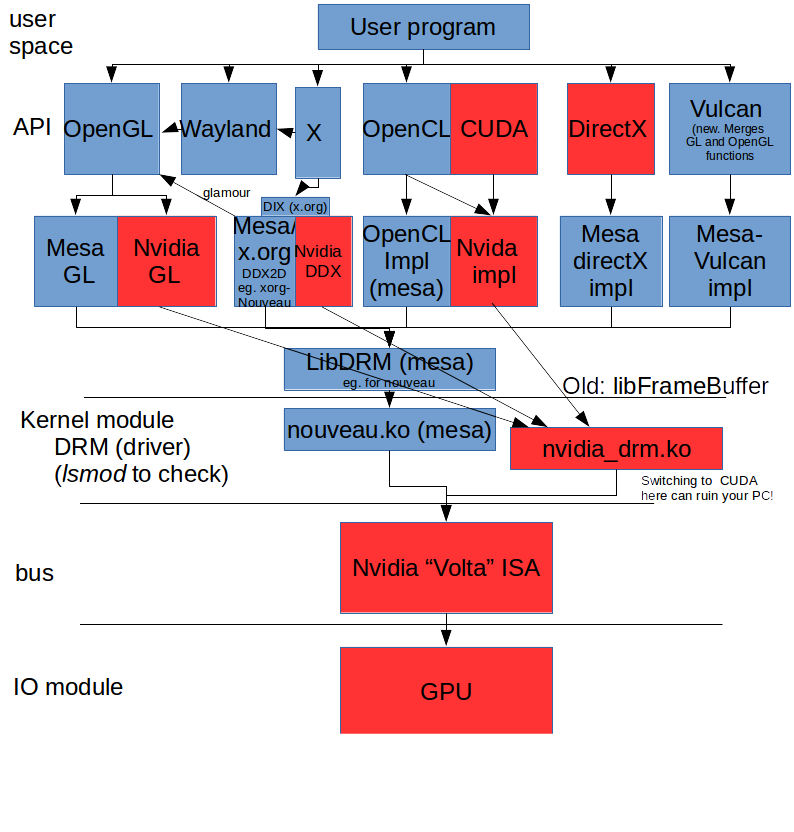
\includegraphics[width=7cm]{figs/graphicsStack.png}
\end{figure}

\section{Further reading}
\url{https://people.freedesktop.org/~marcheu/linuxgraphicsdrivers.pdf}

\url{https://blogs.igalia.com/itoral/2014/07/29/a-brief-introduction-to-the-linux-graphics-stack/}


\chapter{OpenGL (via SDL)}

OpenGL is the industry standard 3D graphics command language.  It provides an API containing commands which draw triangles and linesin 3D space, to render them under different lighting models, and to position the camera geometry around them.

In theory, the OpenGL API can be implemented in all kinds of ways, including fast graphics card hardware to take these commands and render them at blazing speed directly to a monitor. But also, for example, implementations might render drawings from the same commands onto bitmap images, vector graphics canvases, or even to robic spraycan or oil paintbrush manipulators.

Hence, to use the OpenGL requires an implementation library, such as Mesa, and usually a second library which links it to the screen or to a window in the operating system.   We will made use of the SDL (Simple Direct Layer) library as this link here.   SDL provides a graphics context which may be full-screen (eg for writing games) or windowed within the operating system.   


\subsection{SDL}

As modern systems operate from within a desktop window manager, which often gets implemented through OpenGL itself, some method is needed to prepare part of the screen and/or a window in the windowing system for the programmer's own OpenGL commands to run.  This is called a GL context.  It is provided by libraries such as SDL.   The programmer cannot give OpenGL commands directly because the window manager has already bagged the status of "master" of libDRM, and has instructed it not to take commands from anyone else.  SDL is given special permission by the window manager to pass its own commands (via the OpenGL implementations) to libDRM.  libDRM will then see that they coem from an allowed source and let them through to the kernel and GPU.

Simple DirectMedia Layer (SDL) is a cross-platform software development library designed to provide a hardware abstraction layer for computer multimedia hardware components including OpenGL graphics cards, and also keyboards and joysticks.  It is used in 3D games including 0AD, FreeCiv, Oolite, and in 2D games such as Secret Maryo Chnonicles and many others in Humble Bundles.  (Traditionally, a different link library, GLUT, was used. GLUT's programming model requires it to take full control of your program and communicate only through callbacks, while SDL keeps the user in control and assumes they will call its functions regularly. We consider the GLLUT model to be "rude" in takign over control, and this may conflict with other tools which also ask for control, such as ROS.  GLUT is considered old and dying.  Other altneratives include GLFW and pyglet for Python).

\lstinputlisting{snips/sdl_gl/sdlgl.cpp}
\lstinputlisting{snips/sdl_gl/CMakeLists.txt}

GL textures
GL animation

Once you have a context set up, you can apply any GL commands. The classic tutorial on pure GL programming is NeHe's website.  The classic reference is the OpenGL Red Book.

How OpenGL works intenrnall: graphics pipeline: https://fgiesen.wordpress.com/2011/07/01/a-trip-through-the-graphics-pipeline-2011-part-1/

\chapter{SDL 2D graphics and input}
eg for 2d platform games
we are using SDL1.2 (there is newer 2.0 now)

lazyfoo.net

Here is how to blit an image,

\lstinputlisting{/home/charles/Dropbox/linuxMultimedia/snips/sdlImageBlit/lesson01.cpp}

\section{Combining 2D and 3D graphics in SDL}
eg for Augmented Reality overlay!
blit + GL
done by blitting to texture ?

\chapter{Game Engines}
\section{2D}
pygame - built on SDL and OpenAL.  2D scene graph. Collision detection. Partial android version.

\section{3D}
Panda3D - unity-like - developed by Disney?
Blender game engine


\chapter{Cairo vector graphics}

also Pango font rendering ?

\chapter{CAD}
FreeCAD
Blender

\section{Collada (dae) format}


\section{OpenSceneGraph (uses dae)}
B+trees (from GIS book?) - for collision detection

\section{ODE physics engine?}

\chapter{OpenCV}


\section{Reading and writing}

\lstinputlisting{snips/openCVcppCMake/videoWrite.cpp}
\lstinputlisting{snips/openCVcppCMake/CMakeLists.txt}

\section{Basic manipulations}


\chapter{Files and formats}

8 bit colouri = 256 color pallette. Usually with the palette defined in 24 bit in a header. (+ Old VGA has a fixed standard palette)
Standard 24 bit color = 1 byte for each of R,G,B. 32bit adds alpha byte too.  Nice to see and work with, human-readable in hex.

BGR (and ABRG) format for historical reasons. Used by GPU hardware, so libraries like CV follow it for speed.

Various color depths.

"convert" command - very versatile. eg. ps to png.


\section{Data formats}



\subsection{Bitmap (BMP)}

Windows standard. Header then raw RGB array data.

\begin{figure}
	\caption{}
	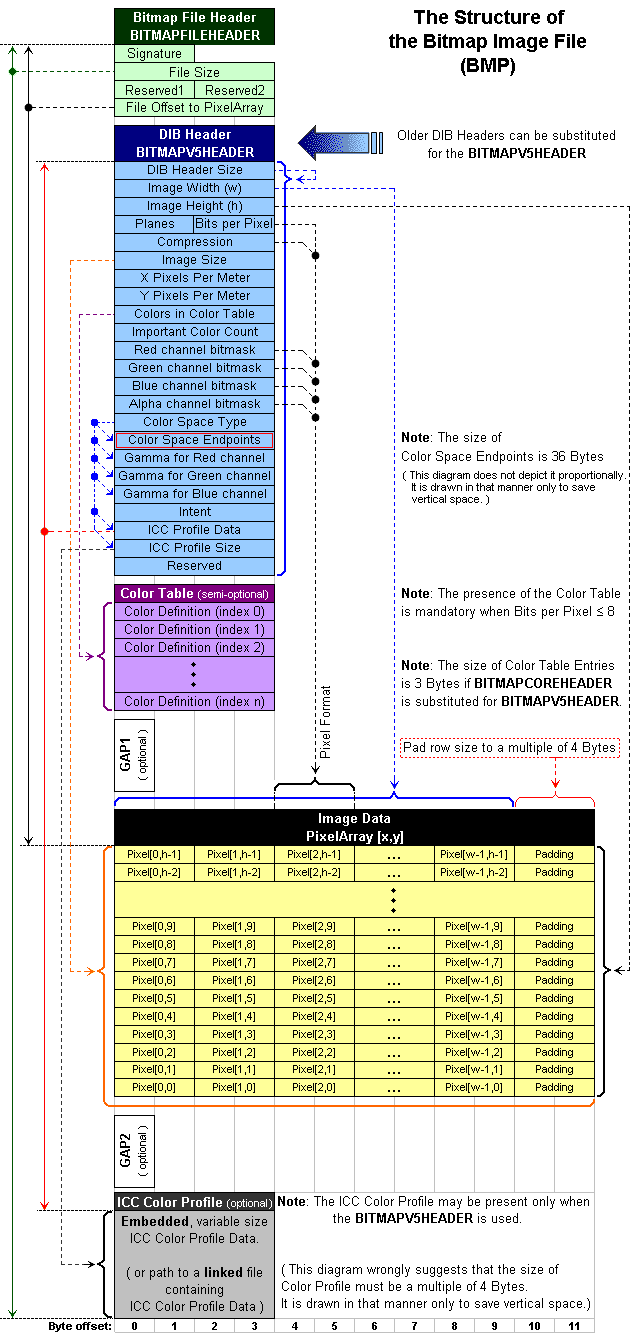
\includegraphics[width=7cm]{figs/BMPfileFormat}
\end{figure}



\section{ROS Image message}

header includes timestamps etc as well as img size and depth.


\section{Portable Network Graphics (PNG)}

compressed, like JPG. File made of chunks of labelled types.


\section{Postscript vector graphics}

as programming language. as used in IOX.


\section{Portable Document Fomat (pdf)}

\lstinputlisting{snips/pdfcut/pdfcut_cmd}



\section{Fonts}


\chapter{GPU OpenCL as graphics programming?}

\section{Architecture}

\section{Low level GPU ISA programming}

It is very rare to program GPUs directly in their own ISA.  Probably the only people who do this are staff at NVidia and staff and volunteers at Mesa who write the implementations for OpenGL and OpenCL etc.

An example program (for an AMD card):

\begin{lstlisting}
00 ALU: ADDR(32) CNT(4) KCACHE0(CB0:0-15)   
0 x: MUL R0.x, KC0[0].x, KC0[1].x    
y: MUL R0.y, KC0[0].y, KC0[1].y
1 z: MUL R0.z, KC0[0].z, KC0[1].z
w: MUL R0.w, KC0[0].w, KC0[1].w
01 EXP_DONE: PIX0, R0
END_OF_PROGRAM
\end{lstlisting}

from:
https://stackoverflow.com/questions/27733704/how-is-webgl-or-cuda-code-actually-translated-into-gpu-instructions

to pass GPU binary via a CL function:
https://www.khronos.org/registry/OpenCL/sdk/1.0/docs/man/xhtml/clCreateProgramWithBinary.html

TODO how to call libDRM directly with the commands ?

\section{OpenCL setup}
We can choose the Mesa stack or a propriatory (eg. NVidia or Intel) stack, for the particular GPU type in our computer.

The Ubuntu nvidia stack can be installed via the Restricted repository, eg. nvidia-opencl-dev gets everything, and replaces the Mesa stack.  Then sudo apt install nvidia-cuda-toolkit to get CUDA and OpenCL APIs, cublas, cudnn, etc.

The mesa stack is harder ...  maybe easier in 16.04 ?
\begin{lstlisting}
/usr/lib/x86_64-linux-gnu/libOpenCL.so.1
\end{lstlisting}
ICD (Installable Client Driver) - Khronos tool to allow multiple implemenations of CL to coexist.
mesa-opencv-icd  apt package ?


\section{OpenCL programming}

Hello world in OpenCL:
\lstinputlisting{snips/cl/go.cpp}
\lstinputlisting{snips/cl/CMakeLists.txt}

(Cmake requres a manual link of libopencl.so.1 to libopencl.so before finding it).

\chapter{Applications}

GIMP

FreeCAD


\part{Audio}


\chapter{How sound cards work}

firewire system (is a bus, chained). FFADO driver (IML setup).
USB system (p2p)


\section{Example: MAUDIO USB card}
    inputs:
	signal dials: -40db control.   Pad: extra -20db.
    flow model:
	all inputs have direct JACK outputs
		the box also has a line out and a phones out
	A/B button-out :patches line out to phones when OUT(A);  
		(spdif to phones when button-in, B)
		so ALWAYS button-OUT if not using any SPDIFs
	Mix: Left: live inputs to phone.  Right: PC to phones
		should be all-right
	Output: volume of line out
	Level: volume of phones
	gtr: inst, vol at 45deg north east

	#NB sampled audio goes out of the MAUDIO through  hw:1,1.  That's nonstanard, defaults are usually hw1,0.  So need to set to listen to hw:1,1.

	#2015: on XPS machine -- need hw2,0 OUTPUT and hw2,1 INPUT (different!)  mich ch 1


\chapter{ALSA (kernel module)}


\section{input}


\section{output}


\chapter{Spatial audio: OpenAL}

\chapter{JACK}

\section{setup}
\url{http://jackaudio.org/faq/linux_rt_config.html}

\begin{lstlisting}
    jackd -d alsa - r48000 -p128 -n2  -P hw:1,0 -C hw:1,1    #works for mic in socket1 of MAUDIO, and for MAUDIIO playboack (not for mic in s2?)

	jackd -dalsa -dhw:0 -r48000 -p128 -n2  #INTERNAL soundcard (not -p64 kills ard3)
	
	killall -9 jackd

qjackctl: (not needed if use JACK cmd above)
	interface (default) (greyed out)
	in dev: hw:1,1
	out dev: hw:1,0	
	chs 2 in 2 out
	128 frames.
\end{lstlisting}

\section{JACK tools}
NB we need to record form the nonstandard hw1,1 , not the default hw1,0:

\begin{lstlisting}
 /usr/bin/jackd -P65 -u -dalsa -r48000 -p128 -n2 -Xseq -D -Chw:1,1 -Phw:1,0 -i2 -o2    #works (and in qjackctl)

killall -9 jackd			#to kill
ecasound -f:16,2,48000 -i jack,system -o rec.wav  			 #record -- not working** (16bit,2ch,48kHz)
ecasound -i output.wav -o jack,system 					 #playback

meterbridge 1   #to open a test app - use qjackctl to connect
\end{lstlisting}


\chapter{LADSPA}


\section{MIDI}

live

files



\chapter{Music notation}

\section{Lilypond file format and engine}
Lilypond names both a format and a program. The program is like Latex for music scores. It creates extremely high-end, professional "engravings" of scores, including fine details equivilent to Latex's kerning and ligatures. Such as tweaking the exact size of note heads and stems, setting stem directions, and hundreds of other small rules passed down from centuries of beautiful score engraving tradition.   The Lilyond program is not an editor and works from a latex-like source file specifying the musical, but not graphical, objects, such as bars, notes, and time signatures. These files can be written by hand or by an editor program such as Denemo (see below). These files do not contain any high level semantic information and they do not show relationships between simultenoys staves (e.g. that a note in one staff is occuring at the saem time as in another) or enable transpoition -- they only represent the low-level musical note content needed for engraving. So you probably don't want to cide directly in LilyPond files. You want to code in some higher level representation then use another program to export it to Lilypond format. 

LilyPond can however do basic transposition from within its code -- usign a transpose command and environment. This is sufficient for quick conversions eg. for Bb jazz isntruments. But not going to be able to do hierarachical stuff.

eg. to write a Schenkerian composition program: use its won format and notation at high level; export to MusicXML; convert to LilyPond; engrave.

Sampel Liypond source:
\lstinputlisting{snips/lilypond/test.ly}

To isntall and compile to pdf:

\begin{lstlisting}
sudo apt-get install lilypond
lilypond test.ly
\end{lstlisting}

Notations:
\begin{lstlisting}
c4 d4 e4 f4  : crochets. 4 means quarter note.
r1 r2 r4 r8  : rests
a4. dotted quarter-note
ds4 : d sharp
a,4 a'4 : octave registers CHANGES. assumes all followign notes in same register.
<c4 e4> : notes together
(c4 e4) : slur notes
\repeat volta 2 { c1 | e1}  : repeat section
c4^"super" e4_"sub" : text above and below note 
\end{lstlisting}

Dynamics are considers as additional over staves.  (LilyPond's name is a pun on an old MIDI editor, RoseGarden).

\section{MusicXML: the interchange format}
Represents scores at a similar level to Lilypond, but is used by many more programs. Specifically there is a MusicXML to Lilypond converter.  It can also be rendered to the pngs used in Wikipedia music pages.  Claims large industry backing (eg. Hollywood score writing commercial systems).

\section{Denemo score editor GUI}
Is designed specifically as a front end to LilyPond, and is to LilyPond as LyX is to Latex.  A what you see if what you mean GUI with its own quick, cheap and chearful interactive graphical screen display, which gets swapped for the advanced engraver when we are done.

(Does not yet export MusicXML but may do soon? CHECK?)

vs - FrescoBaldi - a Lilypond editor which does have MusicXML output? Tis one is not pointy clicky like LyX, is like TexPad, editing the raw lilypond code but with tools to autocompile and display etc.

Includes hum input + assign rhythms to the hummed p[itches

Curosr updown pitch, or type letter name (register nearest to cursor pitch).  Int number keys (use keypad) for durations.



\chapter{File formats}


\section{wav}

header + raw bytes.
NB 4Gb limit? still dont know how to fix this/ repair from header.

\section{vorbis (ogg)}


\chapter{Tools}
\section{Sox and soxi}
Sox is the swiss army knife of the audio command line. Its friend soxi gives information about audio files.
\begin{lstlisting}

	sox k.wav -n stat   #see length(seconds)
	sox in.wav out.wav trim start_time dur			
	sox in.wav out.wav pad start_pad_sec end_pad_sec

	sox ts.wav -b 16 output.wav rate -s -a 48000 dither -s    #upsample
	sox mono.wav -c 2 stereo.wav                              #make stereo fm mono (JACK cares a lot about right types here)

	#delay and weighed mix.  -p is used in place of output fn, to pipe out.
	sox -m -v 0.9 a.wav   -v 0.5 '|sox a.wav -p pad 1' out.wav    #in seconds
	sox -m -v 0.9 a.wav   -v 0.5 '|sox a.wav -p pad 1s' out.wav   #in samples

	#lima
	sox -D -m -v 1 -t sox "|sox a.wav -p pad 0s trim 0 5s"      -v 0.5 -t sox "|sox a.wav -p pad 1s trim 0 5s"  out.wav
 
	#equiv to (as "-p" subs to "-t sox -" and "-" is the pipe out)
	sox  -m -v 1 -t sox "|sox a.wav -t sox - pad 0s trim 0 5s"      -v 0.5 -t sox "|sox a.wav -t sox - pad 1s trim 0 5s"   out.wav
	
	#piping out of sox
	sox -m -v 0.9 a.wav   -v 0.5 '|sox a.wav -p pad 1s' -t wav - | less    #WARNING about wav header though

	#pad and trim
	sox Array1-01.wav -p pad 0s trim 13437440s 104800s  o2.wav

 soxi  /share/spandh.ami1/asr/dev/mtg/ac/exp.mdm/exp/lima/pylima/out/testRun/AMI-S1000B_m4016_083984_084639/iter1/mix.wav

Input File     : '/share/spandh.ami1/asr/dev/mtg/ac/exp.mdm/exp/lima/pylima/out/testRun/AMI-S1000B_m4016_083984_084639/iter1/mix.wav'
Channels       : 1
Sample Rate    : 16000
Precision      : 32-bit
Duration       : 00:00:06.55 = 104800 samples ~ 491.25 CDDA sectors
File Size      : 419k
Bit Rate       : 512k
Sample Encoding: 32-bit Signed Integer PCM

\end{lstlisting}

\section{ALSA command line tools}
\begin{lstlisting}

aplay -D hw:0,0 stereo.wav   #PC
aplay -D hw:0 stereo.wav     #PC
aplay -D hw:1,0 stereo.wav     #USB
aplay -D hw:1,1 stereo.wav     #silent (spdif?)

arecord -f cd -D hw:1,1 g.wav           #works**

\end{lstlisting}

\chapter{Music synthesis}


\chapter{Speech synthesis}

festival


\chapter{Speech recognitions}

kaldi?


\chapter{Applications}

list best LADSPA plugins?

LMMS

\section{Ardour 3}

just create new audio track, should be already to record. 
	(right click in track space, add track)
	(dont need to add audio bus patch) 
	for second and more tracks:
		might need to set to hardware in 1 vs 2
			use icons in top right under "Audio2"

flow model:
	jack,system is conencted auto to the Ardour Master
	the master is connected to any track with record enabled.

region = one segment of wav or midi

SPACE: 		play/stop
SHIFT-SPACE:  	play and record  
SHIFT-R:  	en/diable record (while playing)
(CTL-SPACE: 	stop and forget record)

PUNCH markers are set by ctrl-drag in marker field. 
	Enable puch IN OUT at top right of screen. (under DSP) 
	Press [ to set markers + drag them
	Start record (not just play)
	NB this records NEW WAV FILE doesn't destory old one
 
L: 	en/disable loop play
	works similar to punch, using ] instead of [
	each version is separate WAV, keep old ones	

cursors: 	move to start/end of regions
shift-cursors: 	cue (use spa  ce to stop)
ctl-cursor 	move to marks (CF set, was keypad)

HOME/END goto start/end

6: Auto-Return enable: back to play start location (after play or rec)
7: clicks

to0 SPLIT: select region, position playhead, press S


ARDOUR editing
	S split region at edit pount
	use trim bar (region name area) to crop left and right ends

ARDOUR CONFIGS:
	preferences - default dir

\section{ZynAddSubFX}

musichastie?


\part{Video}


\chapter{Video architecture}

Multimedia comes in various kinds of streams. Streams may contain
video or audio or other things. These may be compressed with codecs,
eg h264,theora. Combining streams eg audio+video is multiplexing.
Demupliplexing is seprate from decoding. Streams can be passed over
realtime protocols such as RTP or stored in container files such as
mp4,ogg. problem with compressing video is that it introduces lateny,
some compressions require knowledge of future frames, eg MP4. Others
are designed for live use eg H264. 

IP cameras - streaming.  vs. save to container files.

\chapter{Video4Linux (V4L)}

is a standard API for video devices such as webcams, plus some drivers
implementing it.

API devices appear as files at ls /sys/class/video4linux/ which can
be accessed eg. via pythonCV: cv2.videoCapture(3) 

v4l2-ctl: gives low level info and setting for USB camera hardware
typically GUI tools are calling into it to change camera settings

has many useful help options, see --help 

get current settings: v4l2-ctl --device=/dev/video0 --get-fmt-video

eg to set image size and codec: v4l2-ctl --device=/dev/video0 --set-fmt-video=width=800,height=600,pixelformat=1

logitech C920 has onboard codecs: YUYV -- splits up luma (Y) and croma
(Cr and Cb red and blue diffs) and downsamples chroma a bit (YUV 4:4:2)
MPEG H264

ask for available frame rates: v4l2-ctl --device=/dev/video0 --list-frameintervals=width=640,height=480,pixelformat=YUYV


\section{Loopback}

Loopback is a system which allows you to create virtual video devices
in V4L, so that other applications may access them just as if they
were real devices. Like real devices they appears in /dev/videoX.

enable kernel module.

create loopback.




\chapter{GStreamer}

linux system for media streams, based on PIPELINEs of modules. (Competitor
to ffmpeg in some ways). Requires modules to go in the pipelines (eg
good/bad/ugly sets, own code). Like \textquotedbl{}ROS for video\textquotedbl{}
? We are using version 1.0 for everything (0.10 also exists) Modules
are binary (Cpp) executables, implementing standard API. (Like LADSPA
- but not as real time? eg including buffering).

includes reading and writing to/from v4l devices. eg. stream things
into new virtual v4l devices for others to read. also UDP data stream
sources and sinks. v4l is a minority sport though as gstreamer has
its own internal appsrc and appsinks.

can give commands to jump to points in streams

it would be a good habit to get used to using gstreamer instead of
ffmpeg for genreal conversion use. it is more powerful for realtime
use and worth knowing.

(\textquotedbl{}!\textquotedbl{} makes the pipe, like unix \textquotedbl{}|\textquotedbl{}
but called a \textquotedbl{}pad\textquotedbl{} rather than \textquotedbl{}pipe\textquotedbl{})

\#basic copy a source file to a sink file: gst-launch-1.0 filesrc
location=\textasciitilde{}/data/qb/NorwichLeeds1280.mp4 ! filesink
location=\textasciitilde{}/out.mp4

\#play mp3 gst-launch-1.0 filesrc location=\textasciitilde{}/test.mp3
! decodebin ! autoaudiosink

\#play mp4 video gst-launch-1.0 filesrc location=\textasciitilde{}/test.mp4
! decodebin ! autovideosink

\#extract a segment of a file, recode, and send to another file (not
working) gst-launch-0.10 gnlfilesource location=\$PWD/source.mp3 start=0
duration=5000000000 media-start=10000000000 media-duration=5000000000
! audioconvert ! vorbisenc ! oggmux ! filesink location=destination.ogg

\#decode a file and stream raw video to a file, gst-launch-1.0 filesrc
location=\textasciitilde{}/test.mp4 ! decodebin ! filesink location=\textasciitilde{}/out.mp4

\#stream to RTP over UDP port gst-launch-1.0 filesrc location=\textasciitilde{}/test.mp4
! decodebin ! x264enc ! rtph264pay ! udpsink host=127.0.0.1 port=9001

\#stream from Ibex robot webcam, to h264 over RTP/UDP. (the comments
tell the other modules about formats which exist at points) gst-launch-1.0
v4l2src ! 'video/x-raw, width=640, height=480, framerate=10/1' ! videoconvert
! x264enc pass=qual quantizer=20 tune=zerolatency ! rtph264pay ! udpsink
host=192.168.0.220 port=1234

\#streaming to a virtual divce is called loopback and it needs to
be enabled: sudo apt-get install v4l2loopback-dkms sudo modprobe v4l2loopback
\#(creates /sys/class/video4linux/video1 and /dev/video1 )

In Ibex, use gstreamer loopback to read an incoming VLC video stream
from the robot eg in RTP format, and create a gstreamer stream here
into V4L. Then python/CV doesn't care what the source was, it just
looks like another webcam. (ffmpeg can also do this?)

We can also do this to stream a video file into gstreamer/loopback(?).
eg. to enable multiple processes to read the same stream and process
it in parallel. gst-launch-0.10 filesrc location=\textasciitilde{}/Documents/my\_video.ogv
! decodebin2 ! ffmpegcolorspace ! videoscale ! ffmpegcolorspace !
v4l2sink device=/dev/video1 (maybe is a bug in gstreamer here)

gst-launch-1.0 -v videotestsrc ! tee ! v4l2sink device=/dev/video1 

\#this works to stream a file over UDP, and read and view it on client:
gst-launch-1.0 filesrc location=\textasciitilde{}/data/qb/NorwichLeeds1280.mp4
! decodebin ! x264enc pass=qual quantizer=20 tune=zerolatency ! rtph264pay
! udpsink host=127.0.0.1 port=9001

gst-launch-1.0 udpsrc port=9001 ! \textquotedbl{}application/x-rtp,
payload=127\textquotedbl{} ! rtph264depay ! avdec\_h264 ! videoconvert
! xvimagesink

\#to read from a V4L port on the same client: (eg then view in VLC)
gst-launch-1.0 udpsrc port=9001 ! \textquotedbl{}application/x-rtp,
payload=127\textquotedbl{} ! rtph264depay ! avdec\_h264 ! videoconvert
! videorate ! video/x-raw, framerate=25/5 ! v4l2sink device=/dev/video1

{*}this works to stream a file into a V4L device: (after activiating
loopback)

sudo modprobe v4l2loopback gst-launch-1.0 filesrc location=\textasciitilde{}/data/qb/NorwichLeeds1280.mp4
! decodebin ! v4l2sink device=/dev/video1

or with some conversions:

gst-launch-1.0 filesrc location=\textasciitilde{}/data/qb/NorwichLeeds1280.mp4
! decodebin ! videoconvert ! videorate ! video/x-raw, framerate=25/5
! v4l2sink device=/dev/video1

PYTHON GSTREAMER API https://github.com/rubenrua/GstreamerCodeSnippets
good tutorials

gst-launch-1.0 rtspsrc location=rtsp://192.168.0.119:88/videoMain !  rtph264depay ! avdec_h264 ! autovideosink

gst-launch-1.0 rtspsrc location=rtsp://192.168.0.119:88/videoMain userid=charles password=PASSWORD !  rtph264depay ! avdec_h264 ! autovideosink



\chapter{ffmpeg}

get video file info ffprobe -show\_streams -i \textasciitilde{}/data/qb/NorwichLeeds1280.mp4

speedup playback of video ffmpeg -r:v \textquotedbl{}480/1\textquotedbl{}
-i sprayingVideo.mp4 -an -r:v \textquotedbl{}12/1\textquotedbl{} output.mp4

split avi into frames: ffmpeg -i corinthian\_raw\_images.avi -f image2
frames/frame-\%3d.png 

extract section: ffmpeg -ss 00:00:05.123 -i in.mp4 -t 00:01:00.00
-c copy out.mp4 \#start time and duration args; can be 00:00:00.000
format, or seconds as 00.000. NB only splits to nearest keyframes
(unless omit copy to transcode)

downsample resolution: ffmpeg -i in.avi -c:a copy -c:v libx264 -crf
23 -s:v 640x360 output.mp4

\begin{lstlisting}
#trimmign with ffmpeg:
ffmpeg -i 140712-g1_s1_10-09-14_c2_45min.avi  -vcodec copy -acodec copy -ss 00:00:00 -t 00:00:04 out.avi

#downsample HD video
ffmpeg -i hd.mts -r 30 -s 960x540 out.mp4
\end{lstlisting}

\chapter{File formats}


\section{theora (ogg)}

\section{AVI}
audio video interleave.  File format containing variously coded audio and video.
	(vs: ogg, mp4-part14(container), asf(AdvancedSystemFormat,Microsfot) )
	can also store other interleaved data, eg subtitles, ubisense data

\section{MP4}

\section{MTS}
MTS is found on portable digital cameras and phones as a video format.  

Here is a conversion method using mencoder:

\begin{lstlisting}
sudo apt-get install build-essential subversion zlib1g-dev
	svn checkout svn://svn.mplayerhq.hu/mplayer/trunk mplayer
	cd mplayer
	./configure
	make
	sudo make install
	mencoder 00001.MTS -o 1.avi -oac copy -ovc lavc -lavcopts vcodec=mpeg4:vbitrate=10000 -fps 50 -vf scale=1920:1080
\end{lstlisting}

\chapter{ROS}

ROS video streams ROS, CV have differerent img formats, use cvbridge
node to convert them: http://wiki.ros.org/cv\_bridge/Tutorials/ConvertingBetweenROSImagesAndOpenCVImagesPython


\chapter{(C)VLC}

STREAMING FROM VLC is maybe easier than gstreamer! To stream a file
as RTP over UDP:

cvlc \textasciitilde{}/data/qb/NorwichLeeds1280.mp4 :sout=\#transcode\{vcodec=h264\}:\textquotedbl{}rtp\{dst=127.0.0.1,port=9001,mux=ts\}\textquotedbl{}

then read from CV with (few seconds delay needed) -- but only by one
client :-( cap = cv2.VideoCapture(\textquotedbl{}udp://@127.0.0.1:9001\textquotedbl{})

multicast: cvlc -vvv \textasciitilde{}/data/qb/NorwichLeeds1280.mp4
:norm=ntsc :v4l2-width=320 :v4l2-height=240 :v4l2-standard=45056 :channel=1
--no-sout-audio --sout '\#transcode\{vb=\textquotedbl{}1600\textquotedbl{},vcodec=mpgv,acodec=mpga,venc=ffmpeg\}:rtp\{proto=udp,mux=ts,dst=127.0.0.1,port=9001\}'
--loop --ttl 

\chapter{Video edit applications}
\section{Openshot}
use openshot program
	import avi , images, make text titles , drag aroudn like cubase
	to crop: select clip, right click, properties, length
	export as avi
	if no clips at start -- shows blank screen (for padding)

\section{Zonemaster}
For CCTV multi IP-camera control.

\section{Desktop recording}
recordmydesktop tool




\part{Multimedia}


\chapter{Containers and streams}

arbitary data streams mixed in. eg robot commands and sensors. Also
subtitles, foreign language audio tracks...

Architecturally -- media streaming is nice as there are no/few branch hazards. Hence DSPs etc.

\chapter{rosbag as a container}


\chapter{H264 (skype, DVDs, mp4s, CCTV cams)}
h264 (aka MP4-part10 (vs just MP4)) is newer format than MP4, used by our IP cameras
	used on Bluray
	they are formats (not suites)


\chapter{H323 (ekiga streams)}
 (ITU) telcon  (signalling)
	is a recommendation (?) to use a whole stack for AV streams:
		RTP (application layer)		
		plus 15 more h. protocols for signalling, resitration, control, all over RTP
		application layer protocols include:
			eg G.711 speech codec, usees VAD to reduce info in quiet bits
			    G.728, linear pred speech coding
			G.722 wideband audio codec
			H.261 an old low res video codec (YouTube, Google Video) (vs MP2,MP4)
			H.263 1996 video codec
			T.127 data exchange during conference
			T.126 image annotation (whiteboard?)
		also included DVB
		(http://www.protocols.com/pbook/h323.htm)

vs Skype format, whichis secret/closed.


\chapter{Real-time transport protocol (RTP) streaming}

RTP is a dedicated http-like protocol, running over UDP (timeliness over reliability), for real time multi media (a media stream format is bit like a container file) usually audio and video.

Application layer (like HTTP, FTP)
	used with RTCP control protocol (quality, syncronisation, monitoring/QoS)
	(RTSP is a higher-level session control protol sometimes used together with RTP, e.g. to give rewind/fast-forward type commands.)
		2010: other transport layers exist for streams, new, eg SCTP stream control

via VLC 

cvlc -vvv v4l2:///dev/video0 --sout '\#transcode\{vcodec=mp2v,vb=800,acodec=none\}:rtp\{sdp=rtsp://:8554/\}' 

cvlc -vvv v4l2:///dev/video0 --sout '\#transcode\{vcodec=h264,vb=800,acodec=none\}:rtp\{sdp=rtsp://:8554/\}'
https://sandilands.info/sgordon/live-webca-streaming-using-vlc-command-line

to read client: 

vlc -vvv --network-caching 200 rtsp://127.0.0.1:8554/

:sout=\#transcode\{vcodec=h264,acodec=mpga,ab=128,channels=2,samplerate=44100\}:rtp\{dst=127.0.0.1,port=5004,mux=ts,sap,name=stream\}
:sout-keep

multicast option


\section{Session Initial Protocol (SIP)}

to set up telcon calls


\chapter{Augmented reality (GL+CV)}

The Graphics Stack architecture above has implications for programs that need to combine 2D and 3D graphics and video, such as head-up displays in 3D games, and augmented reality 3D graphics drawn on top of 2D video camera images.

The best way to do these is to create the image in main RAM in standard (4-byte ABGR, or 3-byte BGR) arrays. Then, like the window manager itself, ask OpenGL to DMA then into GPU texture memory and render them in 3D (using a flat projection matrix). Other 3D graphics can then be drawn over them.  Unlike other image copying, this is a FAST operation due to the DMA implementation.

(Note that GL can render to other buffers inside the graphics card, than the one sent the screen. This is done in souble buffering for example. It is also possible to DMA these buffers back into RAM, eg. if we want to get a rendered image as a sprite and save it to an image file.)

\chapter{Parallel programming}

ROS image format diff frm cv, cvbridge to convert requires ROS stack
overhead ROS kinetic all uses python2, with opencv3 (dont change system
pyton to 3 - kills ROS!) serialise/deserialise and pipe implem,entaion
: serialise is slow. ROS nodelets:allow several nodes to run as a
single process, no msgs.

MPI (network layer 5) wraps all of SYSV/TCPIP/Infiniband python example
message passing, not shmem (some shmem in MPI2?) eg. at each frame,
map (img,dM) across Pool functions to do stuff.

SYSV-python wrapper shmem - after serialisation

GStreamer / V4L app source and sinks stuck on how to get it into opencv/py

RTP/UDP sockets from GStreamer or vlc via GStreamer (http://stackoverflow.com/questions/13564817/python-send-and-receive-rtp-packets)

multiprocessing pipes semaphores shared arrays and map

filelock stuck on a lock

Thrift (over TCP)


\chapter{DSP microprocessors (Texas instruments)}

\chapter{FPGA DSP (verilog, Chisel)}

\chapter{MISC IDEAS}



(DVD uses H.262/MP2 video;  MP2/MP1/AAC audio, all encrypted)

DVB-T Suite used by digital TV (T for terrestrial, also S for satellite and others)
	codecs:
		video: h.264, AVS ...
		audio: mp3, mp2, aac ...


camera cvlc command , to record
	camea is using http to communicate (?) root/88o88o
	resultion request in cgi URL.  Many settings here too.
	save encode format, currently avi/mpeg, 640x400
	480x360, 20fps.
	as URL, shows CCTV monitor :)





\end{document}
